%  article.tex (Version 3.3, released 19 January 2008)
%  Article to demonstrate format for SPIE Proceedings
%  Special instructions are included in this file after the
%  symbol %>>>>
%  Numerous commands are commented out, but included to show how
%  to effect various options, e.g., to print page numbers, etc.
%  This LaTeX source file is composed for LaTeX2e.

%  The following commands have been added in the SPIE class 
%  file (spie.cls) and will not be understood in other classes:
%  \supit{}, \authorinfo{}, \skiplinehalf, \keywords{}
%  The bibliography style file is called spiebib.bst, 
%  which replaces the standard style unstr.bst.  

\documentclass[]{spie}  %>>> use for US letter paper
%%\documentclass[a4paper]{spie}  %>>> use this instead for A4 paper
%%\documentclass[nocompress]{spie}  %>>> to avoid compression of citations
%% \addtolength{\voffset}{9mm}   %>>> moves text field down
%% \renewcommand{\baselinestretch}{1.65}   %>>> 1.65 for double spacing, 1.25 for 1.5 spacing 
%  The following command loads a graphics package to include images 
%  in the document. It may be necessary to specify a DVI driver option,
%  e.g., [dvips], but that may be inappropriate for some LaTeX 
%  installations. 
\usepackage[]{graphicx}
\usepackage{url}
\usepackage[table, xcdraw]{xcolor}
\usepackage{subcaption}

\title{3D scanning by means of dual-projector structured light illumination} 

%>>>> The author is responsible for formatting the 
%  author list and their institutions.  Use  \skiplinehalf 
%  to separate author list from addresses and between each address.
%  The correspondence between each author and his/her address
%  can be indicated with a superscript in italics, 
%  which is easily obtained with \supit{}.

\author{Daniel L. Lau\supit{a} and Ying Yu\supit{a}
\skiplinehalf
\supit{a}University of Kentucky, Address, Lexington, US; \\
%\supit{b}University of Kentucky, Address, Lexington, US
}

%>>>> Further information about the authors, other than their 
%  institution and addresses, should be included as a footnote, 
%  which is facilitated by the \authorinfo{} command.

\authorinfo{Further author information: (Send correspondence to A.A.A.)\\A.A.A.: E-mail: aaa@tbk2.edu, Telephone: 1 505 123 1234\\  B.B.A.: E-mail: bba@cmp.com, Telephone: +33 (0)1 98 76 54 32}
%%>>>> when using amstex, you need to use @@ instead of @
 

%%%%%%%%%%%%%%%%%%%%%%%%%%%%%%%%%%%%%%%%%%%%%%%%%%%%%%%%%%%%% 
%>>>> uncomment following for page numbers
% \pagestyle{plain}    
%>>>> uncomment following to start page numbering at 301 
%\setcounter{page}{301} 
 
  \begin{document} 
  \maketitle 

%%%%%%%%%%%%%%%%%%%%%%%%%%%%%%%%%%%%%%%%%%%%%%%%%%%%%%%%%%%%% 
\begin{abstract}
This document shows the desired format and appearance of a manuscript prepared for the Proceedings of the SPIE.  It contains general formatting instructions and hints about how to use LaTeX.  The LaTeX source file that produced this document, {\tt article.tex} (Version 3.3), provides a template, used in conjunction with {\tt spie.cls} (Version 3.3).  
\end{abstract}

%>>>> Include a list of keywords after the abstract 

\keywords{Manuscript format, template, SPIE Proceedings, LaTeX}

%%%%%%%%%%%%%%%%%%%%%%%%%%%%%%%%%%%%%%%%%%%%%%%%%%%%%%%%%%%%%
\section{INTRODUCTION}
\label{sec:intro}  % \label{} allows reference to this section
Structured light illumination 

\section{HDMI overview}
HDMI is the abbreviation of High-Definition Multimedia Interface, it is one of the most popular display interfaces. The newest release, HDMI Version 2.1 supports up to $10K$ video at $120 Hz$. A standard HDMI connector has 19 pins as listed in Table \ref{Tab:1}.

% Please add the following required packages to your document preamble:
% \usepackage[table,xcdraw]{xcolor}
% If you use beamer only pass "xcolor=table" option, i.e. \documentclass[xcolor=table]{beamer}
\begin{table}[]
\begin{tabular}{|c|l|}
\hline
\rowcolor[HTML]{C0C0C0} 
{\color[HTML]{000000} \textbf{PIN}} & \multicolumn{1}{c|}{\cellcolor[HTML]{C0C0C0}{\color[HTML]{000000} \textbf{DATA}}} \\ \hline
\multicolumn{1}{|l|}{Data2+, Data2 Shield, Data2-} & red pixel component, CTL2, CTL3 and auxiliary data \\ \hline
\multicolumn{1}{|l|}{Data1+, Data1 Shield, Data1-} & green pixel component, CTL0, CTL1 and auxiliary data \\ \hline
\multicolumn{1}{|l|}{Data0+, Data0 Shield, Data0-} & blue pixel component, HSYNC, VSYNC and auxiliary data \\ \hline
\multicolumn{1}{|l|}{Clock+, Clock Shield, Clock-} & pixel clock \\ \hline
SCL, SDA & DDC channel, the source reads the EDID from the sink \\ \hline
CEC & data or commands from remote control \\ \hline
Reserved/HEAC+ & reserved for v1.3 and before, Ethernet and audio since v1.4 \\ \hline
HOT PLUG DETECT/HEAC- & indicate the hot plug or paired with HEAC+ \\ \hline
+5V, Ground & power from external or HDMI source, ground \\ \hline
\end{tabular}\\
\caption{HDMI pinout}
\label{Tab:1}
\end{table}

Data channel 2, 1, 0 are mainly used to transfer red, green and blue components of the video respectively. The HDMI does not only transfer video data, but also some auxiliary data, for example audio data, packet header. The auxiliary data, video data as well as some control signals are encoded in data channel 2, 1, 0 and then digitally transmitted in serial. In between any two adjacent video periods, one or more data island period and control period are inserted. There are six important control signals, HSYNC indicates the beginning and end of a row in a frame of the video, VSYNC indicates the beginning and end of a frame, CTL0~CTL3 indicate the data type of the following data period. The three data channels are transmitted through a differential signaling technology called Transition-Minimized Differential Signaling (TMDS) to reduce the impact of electromagnetic interference and enable high clock skew tolerance. Another common application of TMDS is in the Digital Visual Interface (DVI).\\
The 5 volts power signal is provided by the HDMI source or an external source. After the HDMI sink receives an 5 volts signal at the corresponding pin, it immediately asserts the pin Hot Plug Detect. Once the HDMI source detects the presence of a sink by the assertion of the pin Hot Plug Detect, it sends an $I^2C$-based command of a read request to the sink. The pins SCL and SDA compose the display data channel (DDC) via which the Extended Display Identification Data (EDID) is read by the HDMI source from the sink as the response to the read request. The EDID is usually 128 or 256 bytes long, it contains various information related to the features of display system, including but not limited to, manufacturer ID, serial number, week and year of manufacture, screen size, supported timing, etc.\\
The pin CEC is used to add some advanced functionalities for the HDMI systems. Usually it is a remote control that issues different high-level commands to the devices connected by HDMI cables. CEC stands for Consumer Electronics Control, it is also a one-wire bus protocol, the implementation of CEC is optional, because not all the HDMI devices support this feature. Since HDMI 1.4, the previously reserved pin has become the HDMI Ethernet and Audio Returen Channel (HEAC). While it is in audio return channel mode, only the HEAC+ line is used to transmit audio data; in HDMI Ethernet channel mode, the HEAC+ line pairs up with the HEAC- line as a differential signal to establish a high speed Ethernet communication.

%\begin{figure}
%   \begin{center}
%   \begin{tabular}{c}
%   %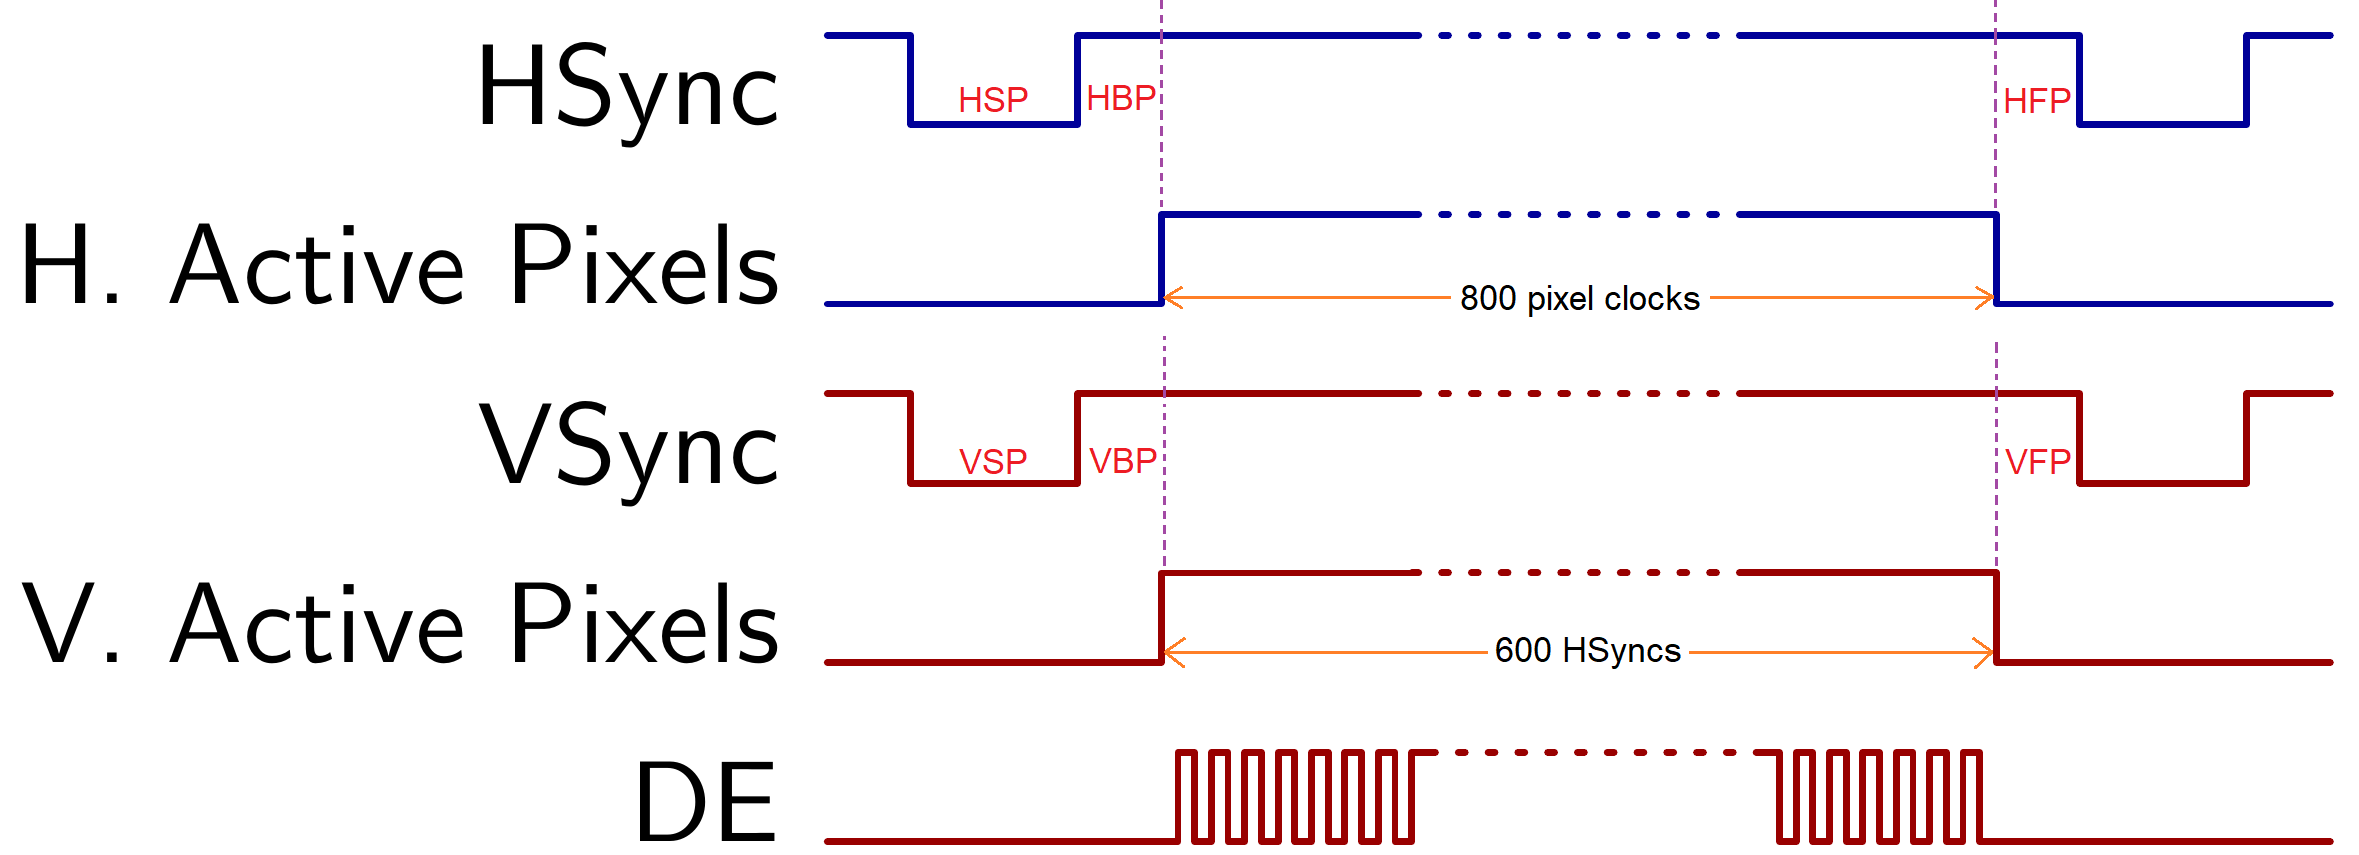
\includegraphics[height=7cm]{wf3.png}
%   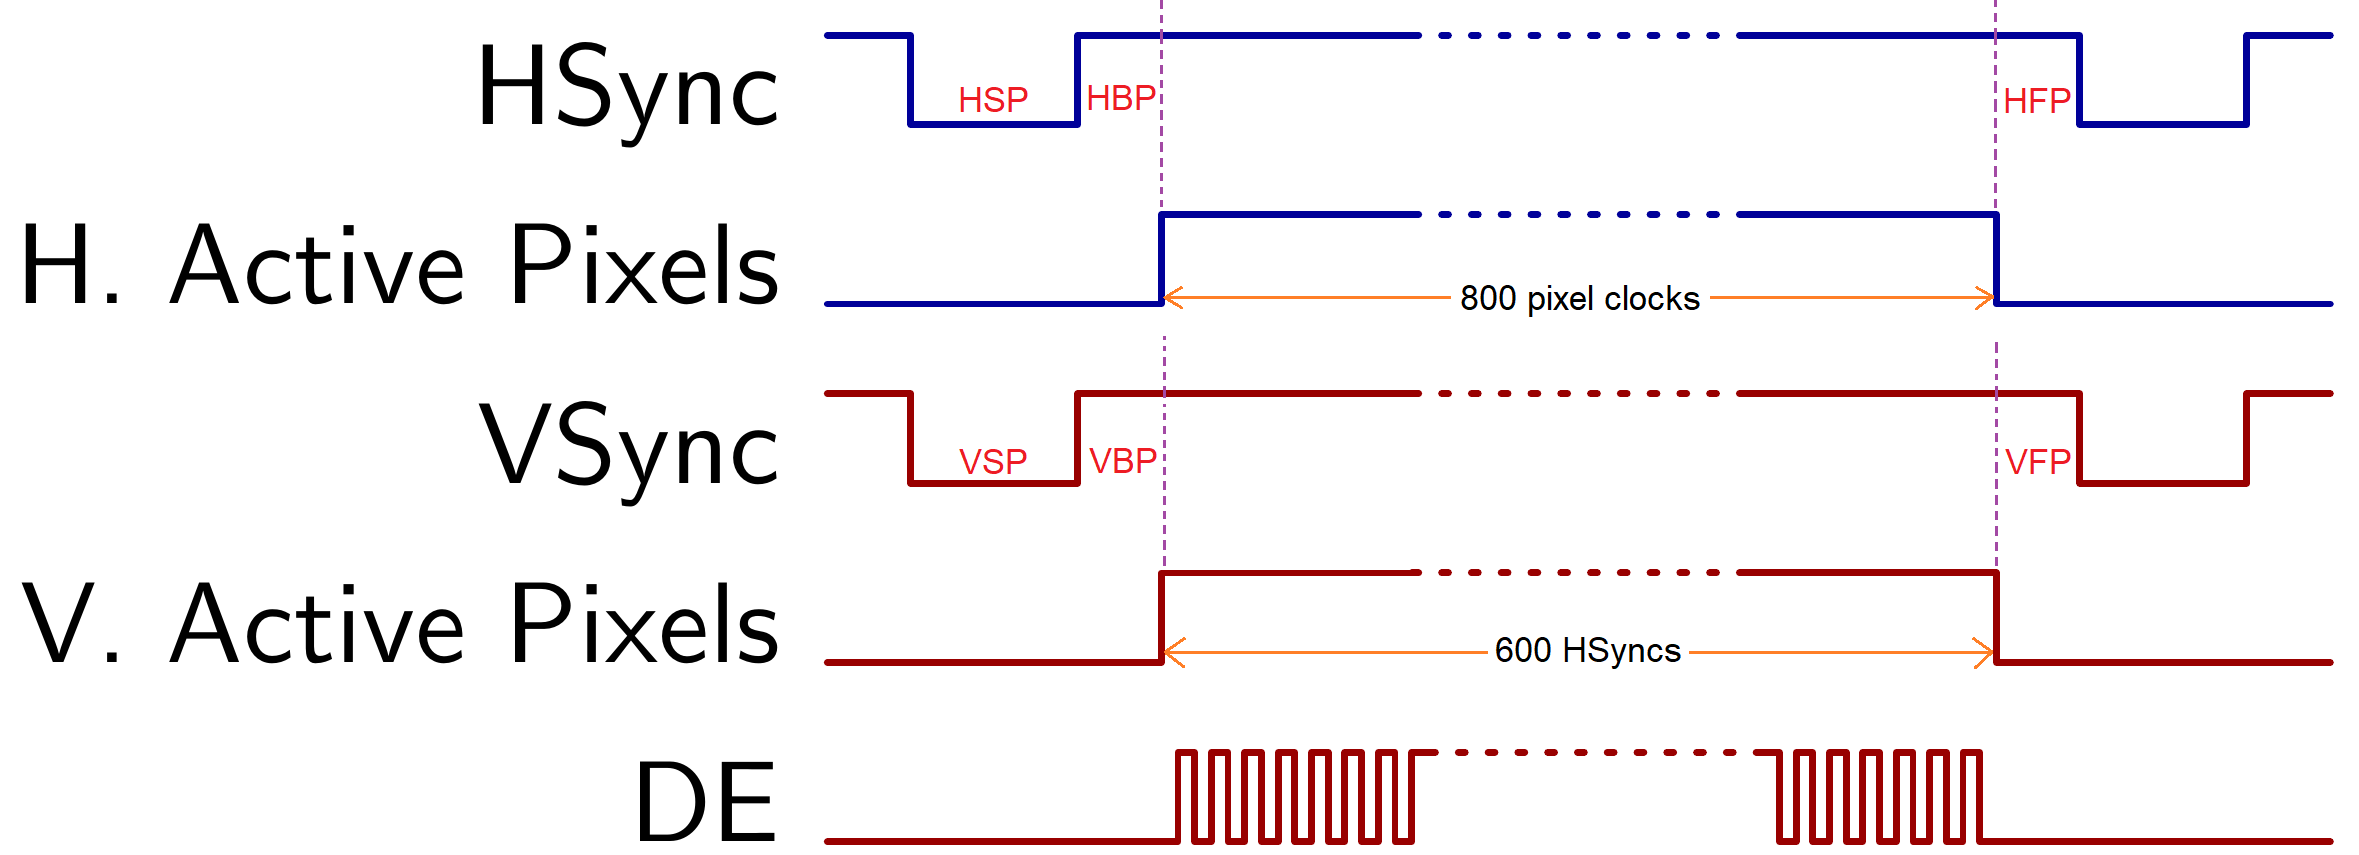
\includegraphics[width=\linewidth]{wf3.png} 
%   \end{tabular}
%   \end{center}
%   \caption{HDMI timing}
%   \label{Fig:1}
%   \end{figure} 

\section{System implementation based on FPGA}
Our FPGA-based dual-projector Structured Light Illumination (SLI) system generates two synchronized SLI patterns which are then fed to two projectors via HDMI. Meanwhile, the projectors and the camera need to be synchronized to ensure that the camera images are taken at the right timing. The system diagram is shown in Figure \ref{Fig:1}.

\begin{figure}
   \begin{center}
   \begin{tabular}{c}
   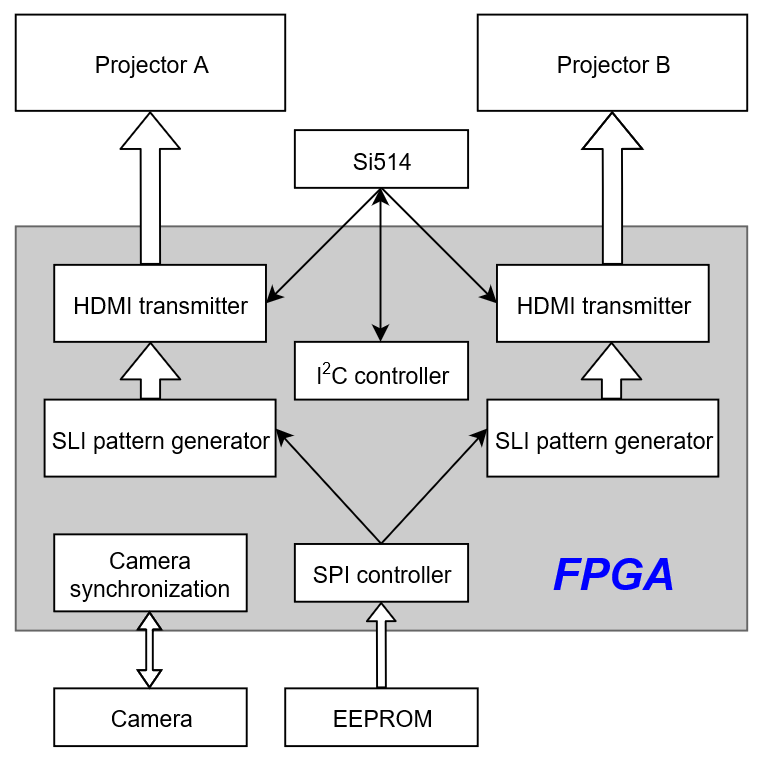
\includegraphics[height=7cm]{sysdg.png}
   %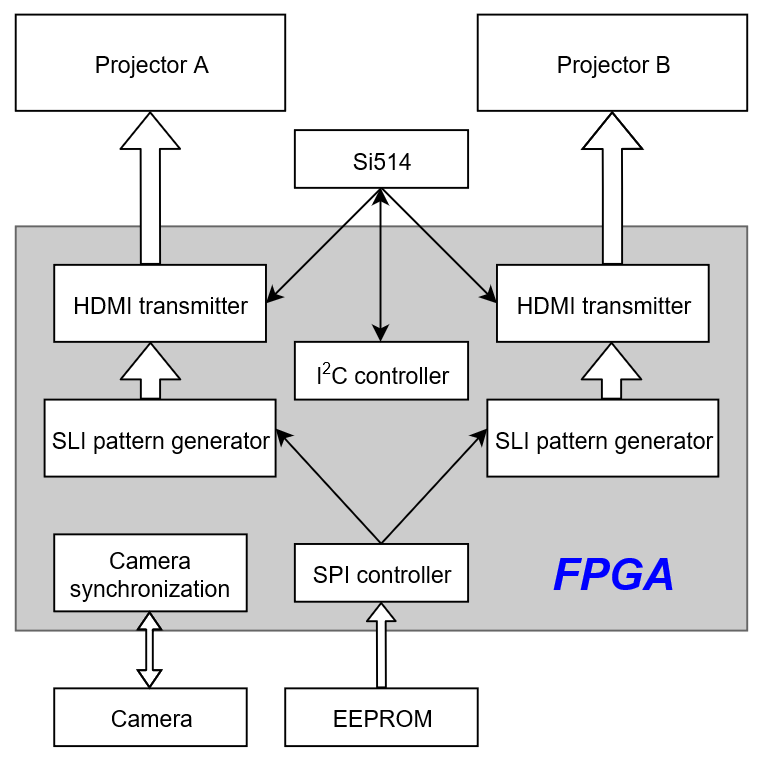
\includegraphics[width=\linewidth]{sysdg.png} 
   \end{tabular}
   \end{center}
   \caption{System diagram}
   \label{Fig:1}
   \end{figure} 

The two SLI pattern generators output two synchronized phase-shifting fringe patterns which are later encoded into TMDS data streams by the HDMI transmitters and eventually move to projectors. The camera synchronization module controls the timing of the camera trigger signal, it detects the end of the camera's exposure time and makes sure that during the whole camera's exposure time, there is no different pattern projected and every unique phase-shifting fringe pattern is pictured sequentially by the camera. The projector in our SLI system operates at the resolution of $800x600$ and the refresh rate of $120 Hz$. According to the document from VESA \cite{vesa07}, the HDMI timing should be set as Table \ref{Tab:2} lists.

\begin{table}[!htb]
\parbox{.45\linewidth}{
\centering
\begin{tabular}{|l|l|}
\hline
\textbf{Pixel Clock} & 73.250MHz \\ \hline
\textbf{Hor. Front Porch} & 48 pixels \\ \hline
\textbf{Hor. Sync Time} & 32 pixels \\ \hline
\textbf{Hor. Back Porch} & 80 pixels \\ \hline
\end{tabular}
}
\hfill
\parbox{.45\linewidth}{
\centering
\begin{tabular}{|l|l|}
\hline
\textbf{Ver. Front Porch} & 3 lines \\ \hline
\textbf{Ver. Sync Time} & 4 lines \\ \hline
\textbf{Ver. Back Porch} & 29 lines \\ \hline
\end{tabular}
}\\
\caption{HDMI timing of $800x600 @ 120 Hz$}
\label{Tab:2}
\end{table}

To obtain the uncommon 73.25MHz pixel clock, we utilize a programmable oscillator Si514. By configuring the internal registers through $I^2C$ bus, Si514 can generate any frequency from 100kHz to 250MHz with a tuning resolution of 0.026 ppb. Therefore, an $I^2C$ master controller was incorporated into the system. One last module in the system is a lookup table (LUT) that is used to linearize the output of the projector. Ideally, the input digital values of the projector is proportional to the light intensity at the output side of the projector. The light intensity is measured by reading the pixel value of the photo taken by the camera. However, in practice, they are non-linear for most of the times due to gamma distortion \cite{}. Introducing a LUT to compensate the gamma distortion is an effective way to address this problem of non-linearity, as shown in the Figure \ref{Fig:2} and Figure \ref{Fig:3}. This LUT can be hard-coded into the configuration file of the FPGA, but the drawback is that once the lookup table changes, the FPGA configuration file has to be changed. It is quite inconvenient especially when the system needs to be often applied to a different projector. We devise a method that the user stores the LUT in an EEPROM which can be erased and written by any computer via serial port or USB, and the SPI master module in the FPGA reads the EEPROM every time the system  is powered on. With this approach, users can load a new LUT much simpler and faster.

\begin{figure}
\centering
\parbox{5cm}{
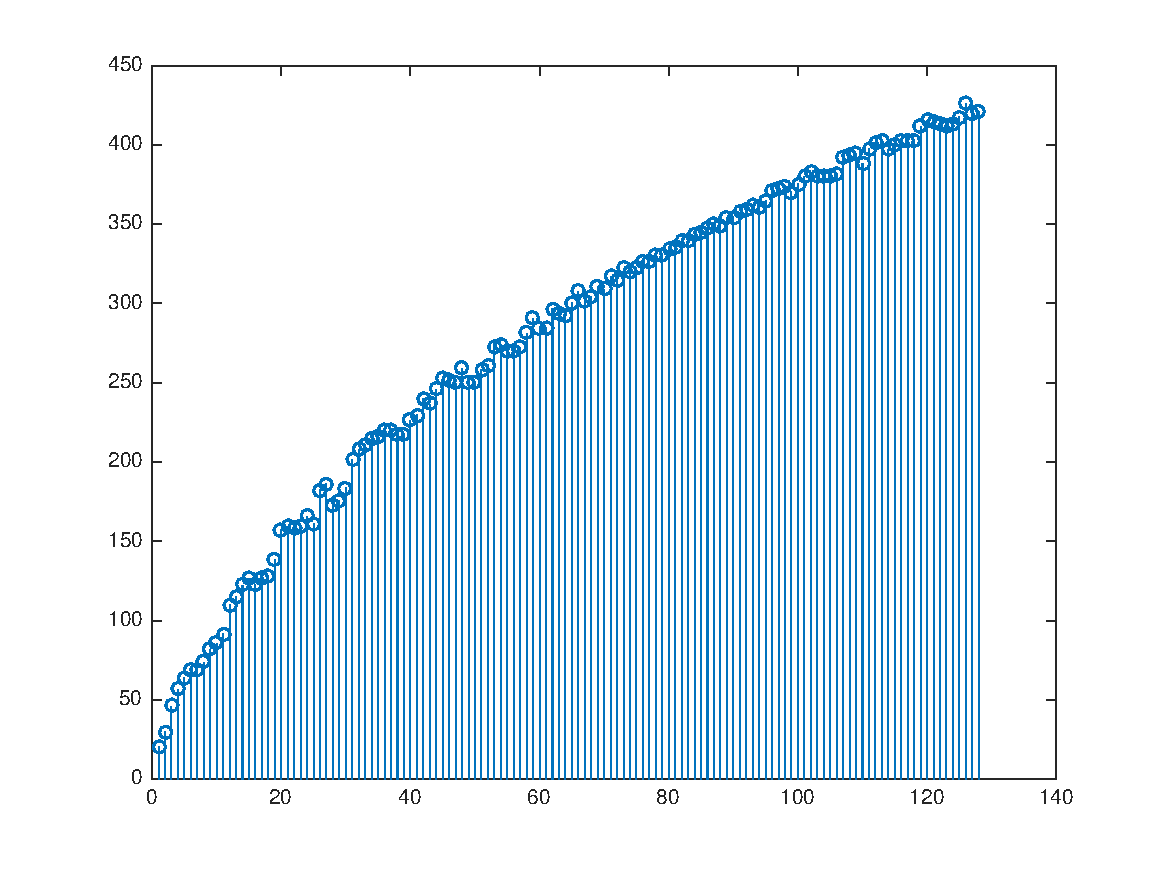
\includegraphics[width=5cm]{lut.pdf}
\caption{output without LUT}
\label{Fig:2}}
\qquad
\begin{minipage}{5cm}
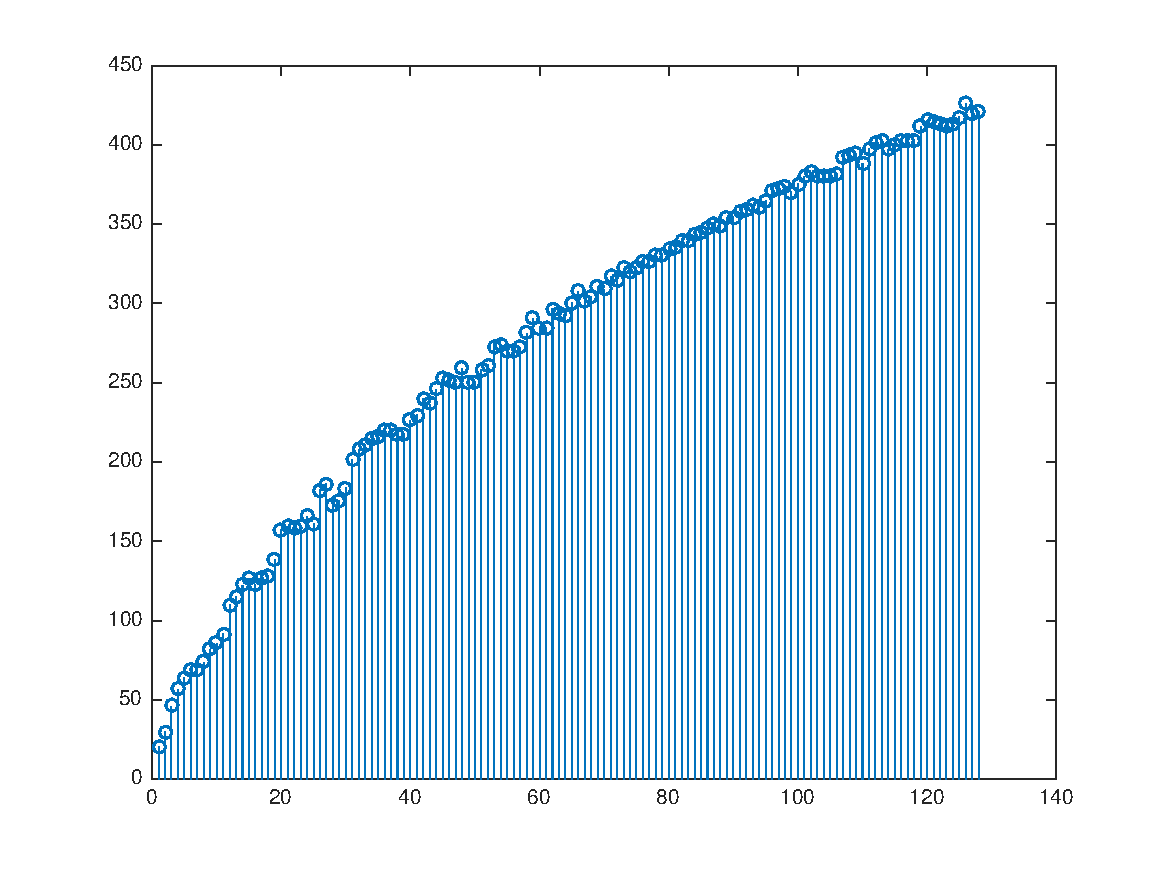
\includegraphics[width=5cm]{lut.pdf}
\caption{output with LUT}
\label{Fig:3}
\end{minipage}
\end{figure}


Our tested system looks as Figure \ref{Fig:3} shows.

\begin{figure}
   \begin{center}
   \begin{tabular}{c}
   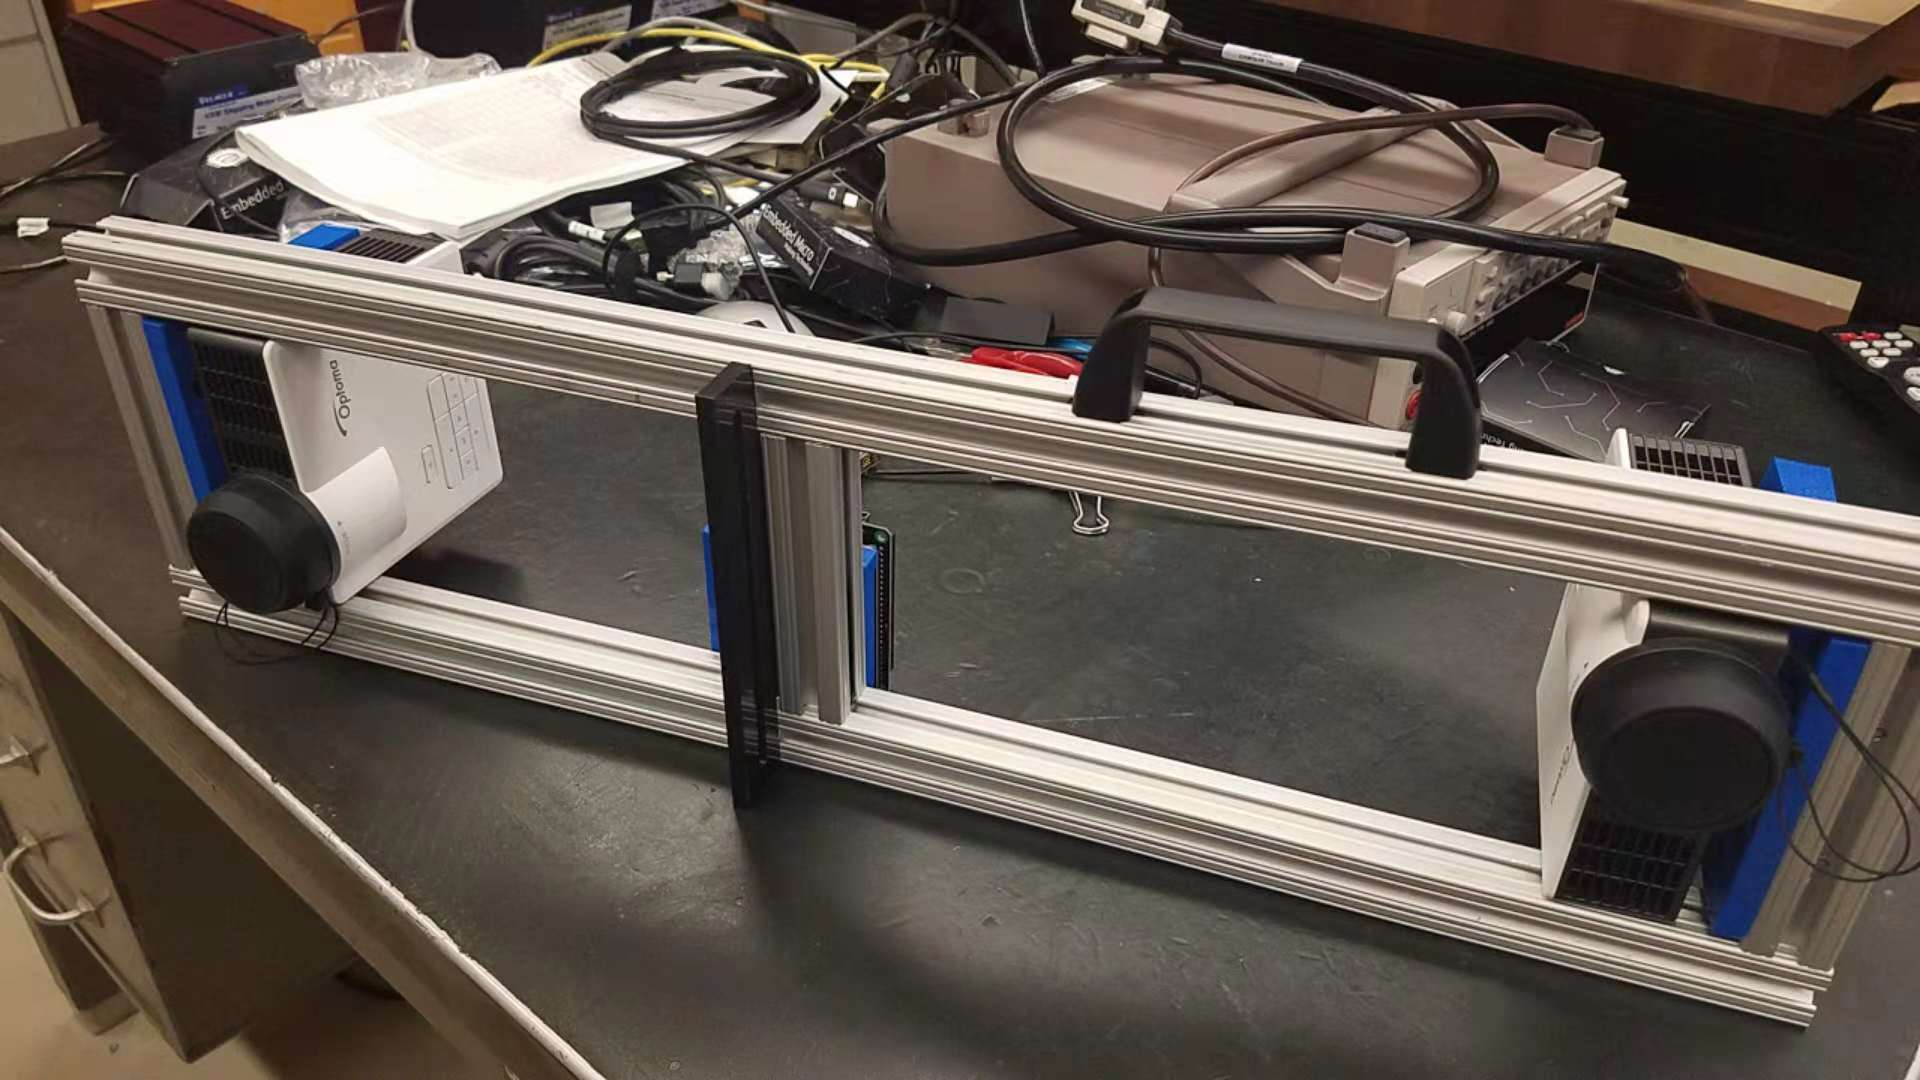
\includegraphics[height=7cm]{dpphoto.jpg}
   %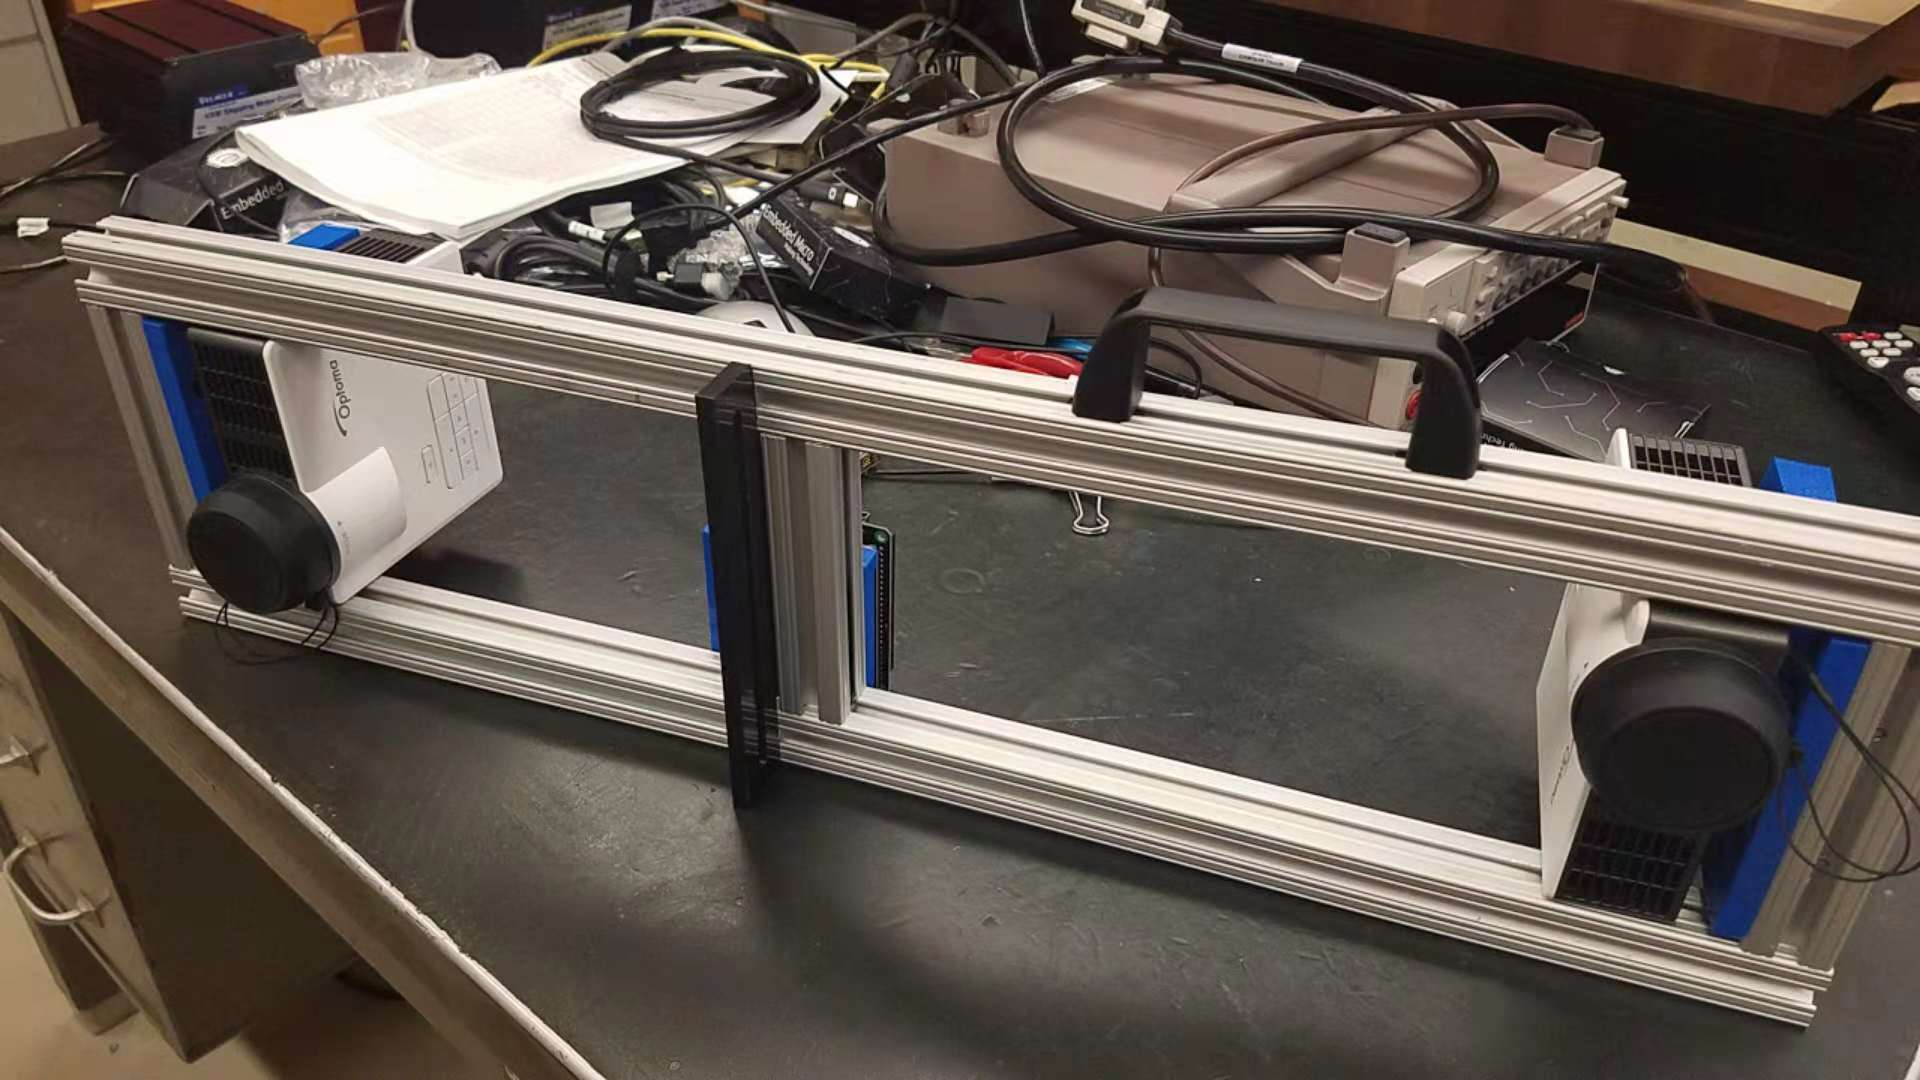
\includegraphics[width=\linewidth]{dpphoto.jpg} 
   \end{tabular}
   \end{center}
   \caption{the dual-projector SLI system}
   \label{Fig:4}
   \end{figure} 

\acknowledgments     %>>>> equivalent to \section*{ACKNOWLEDGMENTS}       
This unnumbered section is used to identify those who have aided the authors in understanding or accomplishing the work presented and to acknowledge sources of funding.  

%%%%%%%%%%%%%%%%%%%%%%%%%%%%%%%%%%%%%%%%%%%%%%%%%%%%%%%%%%%%%
%%%%% References %%%%%

\bibliography{report}   %>>>> bibliography data in report.bib
\bibliographystyle{spiebib}   %>>>> makes bibtex use spiebib.bst

\end{document} 
